\section{Methodology}
The data used in the research comes from the High Performance Manufacturing project (HPM), specifically the fourth round survey. The specific data needed for this research will be gathered in collaboration with Professor Kari Tanskanen.

% \begin{figure}[htbp]
%     \centering
%     \includegraphics[width=\textwidth]{your_figure_file.pdf}
%     \caption{A visualization of the research model}
%     \label{fig:model}
% \end{figure}

Our research methodology is based on \cite{furlanComplementarityLeanManufacturing2011} who used bundles to test for complementarity amongst an aggregate of practices. 
We were also inspired by \cite{maoLowCarbonSupply2017} use of moderating variables to test for more specific environmental effects. 
For the EFA section of the paper we have followed the recommendations provided by \cite{beaversPracticalConsiderationsUsing2013}.
\subsection*{Exploratory Factor Analysis}
The first step of our analysis was to identify the underlying factors of the data, we have a theoritical understanding of the underlying factors of the data, however, we have used exploratory factor analysis (EFA) to first validate our theoritical understanding.
The EFA was conducted using the \texttt{FactorAnalyzer} package for Python \citep{perssonPythonPackagesExploratory2021}.
The EFA was conducted on the various environmental practices, environmental performance and Lean/JIT scales provided in the HPM round 4 dataset.
\\
The EFA was conducted using the minimum residuals extraction method. This was due to the methods flexibility, and the underlying distribution of the data, excluding other methods such as Maximum Likelihood. 
Principal Axis Factoring has not been explored but may also be worth exploring in future research.
We used an oblique rotation method due to the theoritical understanding that the factors will be correlated.
The oblique rotation was conducted using the \texttt{promax} method \texttt{FactorAnalyzer}.
\\
Following \cite{schonrock-ademaNecessaryStepsFactor2009} \& \cite{costelloBestPracticesExploratory2005} we used multiple criteron to determine the number of factors to extract.
This was an iterative process of extracting factors and examining the factor loadings and domain relevance of the factors.
\\
\begin{figure}[htbp]
    \centering
    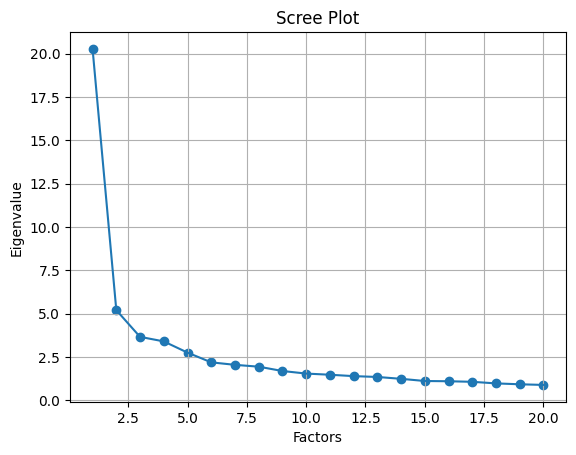
\includegraphics[width=\textwidth]{figures/scree.png}
    \caption{Scree plot indicated an elbow somewhere between 3 and 7 factors}
    \label{fig:model}
\end{figure}
\\
The first method was the Kaiser criterion, which states that factors with eigenvalues greater than 1 should be extracted.
This was first of all not feasable as it produced over 15 factors most of which with very low loadings and little domain relevance, with factors cross loading on multiple variables.
The second method was the scree plot, which is a visual method of determining the number of factors to extract, from this we determined that the elbow was somewhere between 3 and 7 factors (Figure 1). 
\\ 
Working first with seven factors we examined the loadings and domain relevance, we found that the factors had little domain relevace as well as low loadings. Strikingly Factors 5, 6, 7 only contained 3 practices each with loadings above 0.50. (Table 1).
\begin{landscape}
\small
\begin{longtable}{llllllllll}
\caption{Exploratory Factor Analysis - Highlighting loadings > 0.5} \label{tab:EFA} \\
\toprule
HPM Code & Factor 1 & Factor 2 & Factor 3 & Factor 4 & Factor 5 & Factor 6 & Factor 7 & Communality & Uniqueness \\
\midrule
\endfirsthead
\caption[]{Exploratory Factor Analysis - Highlighting loadings > 0.5} \\
\toprule
HPM Code & Factor 1 & Factor 2 & Factor 3 & Factor 4 & Factor 5 & Factor 6 & Factor 7 & Communality & Uniqueness \\
\midrule
\endhead
\midrule
\multicolumn{10}{r}{Continued on next page} \\
\midrule
\endfoot
\bottomrule
\endlastfoot
ENVRTX21 & \cellcolor{yellow}0.53 & 0.15 & -0.0 & 0.13 & -0.15 & 0.2 & -0.02 & 0.387124 & 0.612876 \\
ENVRTX37 & 0.14 & \cellcolor{yellow}0.6 & 0.06 & 0.08 & 0.03 & 0.06 & -0.06 & 0.401213 & 0.598787 \\
ENVRTX02 & \cellcolor{yellow}0.59 & 0.23 & 0.2 & 0.17 & 0.01 & -0.17 & -0.01 & 0.498194 & 0.501806 \\
ENVRTX22 & \cellcolor{yellow}0.6 & 0.14 & 0.23 & 0.1 & -0.15 & 0.13 & -0.07 & 0.490537 & 0.509463 \\
ENVRTX39 & \cellcolor{yellow}0.6 & 0.26 & 0.14 & 0.15 & 0.0 & 0.08 & -0.05 & 0.474416 & 0.525584 \\
ENVRTX23 & \cellcolor{yellow}0.65 & -0.07 & 0.05 & 0.16 & 0.08 & -0.15 & 0.2 & 0.526442 & 0.473558 \\
ENVRTX18 & \cellcolor{yellow}0.53 & 0.42 & 0.05 & 0.15 & 0.19 & 0.04 & -0.02 & 0.515498 & 0.484502 \\
ENVRTX13 & 0.46 & 0.29 & -0.05 & 0.13 & 0.19 & -0.07 & 0.09 & 0.364410 & 0.635590 \\
ENVRTX33 & 0.26 & \cellcolor{yellow}0.62 & 0.16 & 0.02 & -0.03 & 0.09 & 0.02 & 0.493124 & 0.506876 \\
ENVRTX03 & \cellcolor{yellow}0.6 & 0.12 & 0.16 & 0.25 & 0.09 & -0.0 & 0.04 & 0.475674 & 0.524326 \\
ENVRTX20 & \cellcolor{yellow}0.6 & 0.34 & 0.13 & 0.06 & -0.02 & 0.09 & 0.07 & 0.506159 & 0.493841 \\
ENVRTX38 & \cellcolor{yellow}0.6 & 0.36 & 0.15 & -0.0 & 0.07 & 0.01 & 0.15 & 0.546286 & 0.453714 \\
ENVRTX08 & \cellcolor{yellow}0.75 & -0.04 & 0.06 & 0.05 & 0.01 & -0.03 & 0.14 & 0.592730 & 0.407270 \\
ENVRTX05 & \cellcolor{yellow}0.75 & -0.02 & 0.12 & 0.09 & 0.04 & -0.19 & 0.16 & 0.652066 & 0.347934 \\
ENVRTX30 & 0.47 & 0.48 & 0.11 & 0.09 & 0.14 & 0.04 & -0.05 & 0.491478 & 0.508522 \\
ENVRTX24 & \cellcolor{yellow}0.66 & 0.22 & 0.31 & 0.07 & -0.02 & 0.07 & 0.13 & 0.613468 & 0.386532 \\
ENVRTX32 & 0.31 & \cellcolor{yellow}0.68 & 0.2 & 0.03 & -0.04 & 0.14 & -0.07 & 0.633967 & 0.366033 \\
ENVRTX34 & 0.32 & \cellcolor{yellow}0.55 & 0.11 & 0.03 & 0.08 & -0.0 & 0.1 & 0.428647 & 0.571353 \\
ENVRTX04 & \cellcolor{yellow}0.54 & 0.09 & 0.2 & 0.02 & 0.04 & 0.06 & 0.17 & 0.371735 & 0.628265 \\
ENVRTX29 & \cellcolor{yellow}0.55 & \cellcolor{yellow}0.57 & 0.15 & 0.11 & 0.16 & 0.04 & 0.03 & 0.694491 & 0.305509 \\
ENVRTX41 & 0.5 & 0.49 & 0.2 & -0.01 & 0.24 & 0.16 & -0.03 & 0.616388 & 0.383612 \\
ENVRTX40 & 0.46 & \cellcolor{yellow}0.54 & 0.23 & -0.01 & 0.07 & 0.21 & 0.04 & 0.609872 & 0.390128 \\
ENVRTX09 & \cellcolor{yellow}0.56 & 0.35 & 0.18 & 0.16 & 0.1 & 0.04 & -0.04 & 0.516182 & 0.483818 \\
ENVRTX17 & 0.29 & 0.5 & 0.31 & 0.11 & -0.11 & 0.13 & 0.15 & 0.490870 & 0.509130 \\
ENVRTX07 & 0.45 & 0.31 & 0.28 & 0.08 & -0.0 & 0.09 & 0.05 & 0.388896 & 0.611104 \\
ENVRTX11 & 0.47 & 0.43 & 0.18 & 0.1 & 0.14 & 0.2 & -0.07 & 0.513124 & 0.486876 \\
ENVRTX10 & 0.44 & 0.47 & 0.18 & 0.16 & 0.23 & 0.17 & -0.07 & 0.554014 & 0.445986 \\
ENVRTX01 & 0.47 & 0.13 & 0.26 & 0.1 & -0.06 & 0.16 & 0.19 & 0.377254 & 0.622746 \\
ENVRTX14 & \cellcolor{yellow}0.69 & 0.2 & 0.03 & 0.06 & 0.22 & -0.05 & 0.07 & 0.576579 & 0.423421 \\
ENVRTX15 & \cellcolor{yellow}0.64 & 0.25 & 0.01 & 0.07 & 0.17 & -0.16 & 0.14 & 0.546207 & 0.453793 \\
ENVRTX12 & 0.27 & 0.04 & 0.13 & 0.11 & 0.02 & 0.02 & \cellcolor{yellow}0.78 & 0.710872 & 0.289128 \\
ENVRTX31 & 0.29 & \cellcolor{yellow}0.51 & 0.19 & 0.18 & -0.1 & -0.06 & 0.37 & 0.560730 & 0.439270 \\
ENVRTX35 & 0.17 & \cellcolor{yellow}0.67 & 0.06 & 0.2 & 0.02 & -0.21 & 0.23 & 0.621047 & 0.378953 \\
ENVRTX36 & 0.1 & \cellcolor{yellow}0.69 & 0.22 & 0.19 & 0.08 & -0.08 & 0.13 & 0.597819 & 0.402181 \\
ENVRTX06 & 0.5 & 0.02 & 0.26 & -0.01 & 0.08 & -0.01 & 0.32 & 0.434361 & 0.565639 \\
EPRACX01 & 0.23 & 0.12 & 0.08 & 0.05 & 0.01 & 0.23 & \cellcolor{yellow}0.81 & 0.781392 & 0.218608 \\
EPRACX02 & 0.5 & 0.08 & 0.2 & -0.0 & 0.06 & 0.1 & \cellcolor{yellow}0.6 & 0.659780 & 0.340220 \\
EPRACX03 & \cellcolor{yellow}0.62 & 0.11 & 0.31 & 0.05 & -0.09 & 0.16 & 0.17 & 0.557559 & 0.442441 \\
EPRACX04 & \cellcolor{yellow}0.58 & 0.31 & 0.25 & 0.06 & -0.03 & 0.35 & 0.06 & 0.624820 & 0.375180 \\
EPRACX05 & \cellcolor{yellow}0.53 & 0.28 & 0.21 & 0.17 & -0.12 & 0.37 & 0.08 & 0.586183 & 0.413817 \\
EPRACX06 & \cellcolor{yellow}0.52 & 0.36 & 0.21 & 0.16 & 0.02 & 0.27 & -0.03 & 0.539612 & 0.460388 \\
EPERFX01 & 0.37 & 0.17 & \cellcolor{yellow}0.62 & 0.05 & 0.09 & -0.04 & 0.14 & 0.585140 & 0.414860 \\
EPERFX02 & 0.25 & 0.31 & \cellcolor{yellow}0.65 & 0.11 & 0.06 & 0.11 & -0.07 & 0.609480 & 0.390520 \\
EPERFX03 & 0.21 & 0.23 & \cellcolor{yellow}0.78 & 0.13 & 0.09 & -0.13 & -0.06 & 0.747198 & 0.252802 \\
EPERFX04 & 0.17 & 0.16 & \cellcolor{yellow}0.78 & 0.12 & 0.08 & -0.13 & -0.03 & 0.705412 & 0.294588 \\
EPERFX05 & 0.21 & 0.1 & \cellcolor{yellow}0.78 & 0.05 & 0.03 & 0.04 & 0.04 & 0.668555 & 0.331445 \\
EPERFX06 & 0.05 & 0.02 & \cellcolor{yellow}0.73 & 0.07 & -0.02 & 0.01 & 0.11 & 0.550325 & 0.449675 \\
EPERFX07 & 0.18 & 0.2 & \cellcolor{yellow}0.62 & 0.13 & 0.09 & 0.13 & 0.05 & 0.501326 & 0.498674 \\
EPERFX08 & 0.26 & 0.11 & \cellcolor{yellow}0.52 & 0.07 & 0.11 & 0.11 & 0.2 & 0.418796 & 0.581204 \\
EPERFX09 & 0.15 & 0.02 & \cellcolor{yellow}0.52 & 0.1 & -0.02 & -0.01 & 0.09 & 0.312394 & 0.687606 \\
LAYOUTN01 & 0.16 & -0.01 & 0.09 & \cellcolor{yellow}0.69 & 0.04 & -0.02 & 0.06 & 0.514815 & 0.485185 \\
LAYOUTN02 & 0.22 & 0.06 & 0.1 & \cellcolor{yellow}0.66 & -0.07 & 0.08 & -0.04 & 0.503373 & 0.496627 \\
LAYOUTN03 & 0.12 & 0.18 & 0.05 & \cellcolor{yellow}0.65 & -0.07 & 0.04 & 0.07 & 0.485319 & 0.514681 \\
LAYOUTN04 & 0.18 & 0.09 & 0.06 & \cellcolor{yellow}0.6 & 0.01 & 0.25 & 0.02 & 0.473988 & 0.526012 \\
JITDELN01 & 0.08 & 0.17 & 0.19 & 0.27 & 0.34 & 0.39 & 0.06 & 0.414861 & 0.585139 \\
JITDELN02 & 0.0 & 0.18 & 0.26 & 0.03 & 0.33 & 0.26 & -0.01 & 0.278420 & 0.721580 \\
JITDELN03 & -0.02 & 0.24 & 0.14 & 0.29 & 0.32 & 0.23 & -0.05 & 0.316878 & 0.683122 \\
KANBANN01 & -0.04 & 0.11 & 0.01 & -0.0 & 0.15 & \cellcolor{yellow}0.51 & 0.1 & 0.306588 & 0.693412 \\
KANBANN02 & 0.06 & -0.03 & -0.06 & 0.25 & 0.15 & \cellcolor{yellow}0.55 & 0.05 & 0.399152 & 0.600848 \\
KANBANN03 & 0.09 & -0.04 & -0.04 & 0.18 & 0.2 & \cellcolor{yellow}0.67 & 0.04 & 0.530976 & 0.469024 \\
LINKCN01 & 0.2 & -0.02 & 0.13 & 0.28 & \cellcolor{yellow}0.54 & 0.27 & -0.01 & 0.500219 & 0.499781 \\
LINKCN02 & 0.09 & -0.07 & 0.04 & 0.42 & 0.3 & 0.01 & 0.11 & 0.294498 & 0.705502 \\
LINKCN03 & -0.01 & -0.01 & 0.08 & 0.48 & 0.37 & -0.01 & -0.04 & 0.377006 & 0.622994 \\
LINKCN04 & 0.05 & 0.06 & 0.0 & 0.23 & \cellcolor{yellow}0.73 & 0.13 & 0.05 & 0.616880 & 0.383120 \\
LINKCN05 & 0.08 & 0.09 & 0.02 & 0.21 & \cellcolor{yellow}0.74 & 0.29 & 0.04 & 0.689089 & 0.310911 \\
SCHEDN01 & 0.05 & 0.07 & 0.04 & \cellcolor{yellow}0.59 & 0.15 & 0.1 & 0.08 & 0.395107 & 0.604893 \\
SCHEDN02 & 0.01 & 0.09 & 0.03 & \cellcolor{yellow}0.6 & 0.15 & 0.1 & 0.05 & 0.402938 & 0.597062 \\
SCHEDR03 & 0.07 & -0.21 & 0.09 & -0.05 & -0.14 & -0.15 & -0.0 & 0.103053 & 0.896947 \\
SETUPN01 & 0.17 & 0.05 & 0.02 & \cellcolor{yellow}0.53 & 0.12 & 0.0 & 0.01 & 0.324477 & 0.675523 \\
SETUPN02 & -0.04 & 0.18 & 0.16 & \cellcolor{yellow}0.57 & 0.04 & 0.05 & -0.04 & 0.390410 & 0.609590 \\
SETUPN03 & 0.17 & 0.21 & 0.15 & 0.46 & 0.35 & 0.02 & -0.09 & 0.435804 & 0.564196 \\
\end{longtable}

\end{landscape}
We then reduced the number of factors to 6 and then 5, and found that the factors had a higer domain relevant and had higher loadings, but still faced many cross loading issues especially with the Lean/JIT groups.
The domain relevance of these factors are also questionable as JIT was broken down into multiple factors with insufficient loadings to build a domain relevant factor.
Eventually we settled on 4 factors, which had high loadings and were domain relevant, revealing a domain relevant breakdown of the environmental practices while retaining the domain relevance of the Lean/JIT and enviromental performance groups.
3 factors also had high loadings and domain relevance, but as we had no reason to reject the breakdown in environmental practices suggested by the EFA we decided to continue with 4 factors. See Table 2, 3, 4 \& 5 below for a breakdown of our final bundles.
\begin{table}[htbp]
\centering
\caption{Environmental Practices 1 (General)}
\label{tab:your_label}
\begin{tabular}{lll}
\toprule
HPM Code & Description & Loadings \\
\midrule
ENVRTX08 & Decreasing Environmental Accident Impact & 0.851406 \\
ENVRTX05 & Pollution Prevention & 0.846418 \\
ENVRTX23 & Environmental Improvements for Scrap/Excess Materia... & 0.775964 \\
EPRACX02 & Internal Environmental Management Procedures & 0.671973 \\
ENVRTX14 & Industry-wide Code Compliance & 0.653831 \\
ENVRTX15 & Plant Compliance/Auditing Program & 0.629963 \\
EPRACX03 & Cleaner Production Technologies & 0.601676 \\
ENVRTX24 & Environmental Improvements for Equipment Dispositio... & 0.596048 \\
\bottomrule
\end{tabular}
\end{table} \\
\begin{table}[htbp]
\centering
\caption{Environmental Practices 2 (Suppliers)}
\label{tab:your_label}
\begin{tabular}{lll}
\toprule
HPM Code & Description & Loadings \\
\midrule
ENVRTX32 & Purchasing from M/WBE Suppliers & 0.823226 \\
ENVRTX33 & Formal M/WBE Supplier Purchase Program & 0.721714 \\
ENVRTX37 & Third Party Monitoring of Supplier Working Conditio... & 0.703129 \\
ENVRTX36 & Asking Suppliers for Living Wage & 0.662381 \\
ENVRTX29 & Encouraging Supplier Environmental Improvement & 0.641546 \\
ENVRTX40 & Co-development with Suppliers for Environmental Imp... & 0.620094 \\
ENVRTX34 & Ensuring No Sweatshop Labor in Supplier Plants & 0.605227 \\
ENVRTX35 & Ensuring Supplier Child Labor Law Compliance & 0.600539 \\
\bottomrule
\end{tabular}
\end{table} \\
\begin{table}[htbp]
\centering
\caption{JIT Practices}
\label{tab:your_label}
\begin{tabular}{lll}
\toprule
HPM Code & Description & Loadings \\
\midrule
LINKCN05 & Our customers are linked with us via JIT systems. & 0.623435 \\
SCHEDN02 & We usually complete our daily schedule as planned. & 0.621872 \\
SCHEDN01 & We usually meet the production schedule each day. & 0.619473 \\
LINKCN03 & We can adapt our production schedule to sudden prod... & 0.609956 \\
LINKCN04 & Our customers have a pull type link with us. & 0.594620 \\
LINKCN01 & Our customers receive just-in-time deliveries from ... & 0.592328 \\
LAYOUTN01 & Equipment Layout - Proximity & 0.591347 \\
LAYOUTN04 & Equipment Layout - JIT Production & 0.579354 \\
\bottomrule
\end{tabular}
\end{table} \\
\begin{table}[htbp]
\centering
\caption{Environmental Performance}
\label{tab:your_label}
\begin{tabular}{lll}
\toprule
HPM Code & Description & Loadings \\
\midrule
EPERFX06 & Releases to Water & 0.812363 \\
EPERFX04 & Water Consumption & 0.810310 \\
EPERFX05 & Emissions to Air & 0.804205 \\
EPERFX03 & Energy Consumption & 0.784988 \\
EPERFX02 & Raw Materials Consumption & 0.608603 \\
EPERFX07 & Solid Waste Generation & 0.607016 \\
EPERFX01 & Overall Environmental Performance & 0.584450 \\
EPERFX09 & Fines or Violations & 0.543801 \\
\bottomrule
\end{tabular}
\end{table} \\\\
\begin{table}[htbp]
\centering
\caption{Variance Explained by EFA}
\label{tab:your_label}
\begin{tabular}{llll}
\toprule
Factor & Eigenvalue & Variance Explained \% & Cumulative Variance Explained \% \\
\midrule
Factor 1 & 20.274239 & 26.770974 & 26.770974 \\
Factor 2 & 5.197752 & 6.296780 & 33.067754 \\
Factor 3 & 3.654683 & 4.362066 & 37.429821 \\
Factor 4 & 3.393518 & 3.945660 & 41.375481 \\
Factor 5 & 2.746089 & 3.003128 & 44.378609 \\
Factor 6 & 2.184200 & 2.426975 & 46.805584 \\
Factor 7 & 2.040140 & 2.098922 & 48.904506 \\
\bottomrule
\end{tabular}
\end{table} \\\\
One remaining point on the EFA process recommended by \citep{beaversPracticalConsiderationsUsing2013} is to check the amount of variance explained by the factors.
We found that the 4 factor model explained ~41\% of the variance in the data, while the 7 factor model explained ~49\% of the variance in the data.
Due to the lack of interpretability of the 7 factor model and above models we decided to continue with the 4 factor model. (Table 6)
\\
Although \citep{furlanComplementarityLeanManufacturing2011} used a CFA to identify the factors, we have used an EFA to identify smaller bundles and validate theoretical assumptions. We also performed a CFA based on the relevant HPM round 4 scales. The results of the CFA analysis are included in the appendix.
\subsection*{Complimentarity Analysis}
The first step in the complimentarity analysis as demonstrated by \citep{furlanComplementarityLeanManufacturing2011} was to create a dummy variable for each bundle based on the factors.
Dummy variables were created for each bundle, with the dummy variable being 1 if the firm scored above the median on all practices in the bundle, and 0 otherwise.
From these 4 categories were constructed based on the combinations of bundles, these categories are:
\begin{itemize}
    \item High JIT \& Environmental
    \item Low JIT \& Environmental
    \item Mainly Environmental
    \item Mainly JIT
\end{itemize}
See table 7 below for a breakdown of the categories.
\begin{table}[htbp]
    \centering
    \caption{Frequency of Adoption and Environmental Performance}
    \label{tab:your_label}
    \begin{tabular}{lrll}
\toprule
Category & Frequency & Percentage & Mean of Performance \\
\midrule
High JIT \& Environmental & 57 & 32.57 & 3.91 \\
Mainly Environmental & 38 & 21.71 & 3.78 \\
Mainly JIT & 40 & 22.86 & 3.58 \\
Low JIT \& Environmental & 40 & 22.86 & 3.28 \\
\bottomrule
\end{tabular}

    \end{table}
    
The next step was to conduct a Tukey HSD test to determine if there was a significant difference between the mean environmental performance of the four groups.
The results of the Tukey HSD test will be discussed in the results section.
\subsection*{Regression Analysis}
The final step in the analysis was to conduct a regression analysis to determine if there was a significant moderating effect of JIT on the relationship between environmental practices and environmental performance.
The regression analysis was conducted using the \texttt{statsmodels} package for Python \citep{seaboldStatsmodelsEconometricStatistical2010}.
